\section{Syntax of \lang{}}
\label{sec:syntax}

In this section, we introduce the syntax of \lang{}. A \lang{} program, as shown in the following block, essentially contains several parts,
\begin{bnf}
    \ntsym{program} ::=  (& \ntsym{typedef} | \ntsym{function} | \ntsym{automaton} | \ntsym{system})^*
\end{bnf}

% TODO: make it clear
\begin{enumerate}
    \item A \emph{typedef} specifies an alias name for given types.
    \item A \emph{function} defines a customized function that can be reused in other functions, automata and systems.
    \item An \emph{automaton} defines an automaton through local variables and transitions.
    \item A \emph{system} blocks declare a set of components and connections between them. Both components and connections are described by automata.
\end{enumerate}

\subsection{Type System}
\label{subsec:typesystem}
\lang{} provides a rich-featured type system that supports various data types that are widely used in both formal modeling languages and programming languages.

\smalltitle{Primitive Types} Table. \ref{table:primitivetypes} shows the primitive types supported by \lang{} including: \emph{ integers and bounded integers,  real numbers with arbitrary precision, boolean values, single characters (ASCII only) and finite enumerations}.

\begin{table}
    \caption{Primitive Data Types}
    \label{table:primitivetypes}
    \centering
    \begin{tabular}{lcr}
        \hline
        Name & Declaration & Term Example \T\B \\
        \hline
        \T Bounded Integer\hspace{0.5cm} & \texttt{int lowerBound .. upperBound}\hspace{0.5cm} & \texttt{-1,0,1} \\
        Integer & \texttt{int} & \texttt{-1,0,1} \\
        Real & \texttt{real} & \texttt{0.1, 1E-3} \\
        Boolean & \texttt{bool} & \texttt{true, false} \\
        Character & \texttt{char} & \texttt{'a', 'b'} \\
        \B Enumeration & \texttt{enum {item$_1$, ..., item$_n$}} & \texttt{enumname.item} \\
        \hline
    \end{tabular}
\end{table}

\noindent\emph{Composite Types.} Composite types can be used to contruct complex data types from simpler ones. Several composite patterns are introduced as follows,

\begin{table}
    \caption{Composite Data Types (\texttt{T} denotes an arbitrary data type)}
    \centering
    \begin{tabular}{lr}
        \hline
        Name & Declaration \T\B \\
        \hline
        \T Tuple  & \texttt{T$_1$,...,T$_n$ }\\
        Union & \texttt{T$_1$|...|T$_n$ } \\
        Array & \texttt{T [length]}\\
        Slice & \texttt{T []} \\
        Map & \texttt{map [T$_{key}$] T$_{value}$} \\
        Struct\hspace{1cm} & \texttt{struct \{ field$_1$:T$_1$,..., field$_n$:T$_n$ \}} \\
        \B Initialized & \texttt{T$_{base}$ init term} \\
        \hline
    \end{tabular}
\end{table}

\begin{itemize}
    \item \emph{Tuple}. The \emph{tuple} operator `,' can be used to construct a finite tuple type with several base types.
    \item \emph{Union}. The \emph{union} operator `$|$' is designed to combine \emph{disjoint} types as a more complicated one. 
    \item \emph{Array} and \emph{Slice}. An \emph{array} $T[n]$ is a finite ordered collection containing exactly $n$ elements of type $T$. Moreover, a \emph{slice} is an array of which the capacity is not specified, i.e. slice is a dynamic array.
    \item \emph{Map}. A \emph{map }[$T_{key}$] $T_{val}$ is a dictionary that maps a key of type $T_{key}$ to a value of type $T_{val}$.
    \item \emph{Struct}. A \emph{struct }\{$field_1:T_1,\cdots,field_n:T_n$\} contains $n$ fields, each has a particular type $T_i$ and a unique identifier $field_i$.
    \item \emph{Initialized}. An initialized type is used to specify default value of a term with type $T_{base}$.
\end{itemize}

\noindent\emph{Parameter Types}. In many situations, we need to define a generalizable automaton or system that includes a template function or template component. For example, a binary operator that support various operation ($+$,$\times$, etc.), or an encrypted communication system that supports different encryption algorithms. Parameter types make it able to take functions and components (or systems, of course) as a template parameter. 
\begin{enumerate}
    \item \emph{An Interface}, denoted by \texttt{interface (port$_1$:T$_1$,$\cdots,$port$_n$:T$_n$)}, defines a parameter that could be any \emph{automaton} or \emph{system} that have exactly the same interface (i.e. number, types and directions of the ports are a perfect match). Interfaces are only used in templates of \emph{system}s.
    \item \emph{A Function}, denoted by \texttt{func (arg$_1$:T$_1$,$\cdots, $arg$_n$:T$_n$) : T}, defines a function that have the same argument types and return types. Functions are permitted to show up in templates of \emph{other functions}, \emph{system}s and \emph{automata}.
\end{enumerate}
An example of parameter types can be found in Example. \ref{exp:clustersystem}.

For simplicity, we use $Dom(T)$ to denote the value domain of type $T$, i.e. the set of all possible value of $T$.

\begin{example}[Types Used in a Queue] Queue is a well-known data structure, and it is also used in various message-oriented middlewares. In this example, we introduce some type declarations and local variables used in an automaton \texttt{Queue}. As shown in the following code fragment, we declares a singleton enumeration \texttt{NULL}, which contains only one element \texttt{null}. The buffer of a queue is in turn formalized as an array of \texttt{T} or \texttt{NULL}, indicating that the elements in a queue can be either an assigned item or empty. The head and tail pointers are defined as two bounded integers.
\begin{lstlisting}
typedef enum {null} init null as NULL;
automaton <T:type,size:int> Queue(A:in T, B:out T) {
    variables {
        buf : ((T | NULL) init null) [size];
        phead : int 0 .. (size - 1) init 0;
        ptail : int 0 .. (size - 1) init 0;
    }
    ...
}
\end{lstlisting}
\label{exp:typeinqueue}
\end{example}

\subsection{Functions}
Functions encapsulate complex computing steps and reuse them. In \lang{}, the functions are a bit different from common programming languages -- they include no control statements at all but assignments. This design makes functions' behavior more predictable since it can be resolved into a single formula. For the same reason, functions have access only to its local variables and arguments.

The abstract syntax tree of functions is shown as follows.

\begin{bnf}
    \ntsym{funcDecl} ::= & \tsym{function} \ntsym{template}^? \ntsym{identifier} \tsym{(} \ntsym{arguments} \tsym{)} \tsym{\{} \\
    & (\tsym{variables} \tsym{\{} \ntsym{varDecl}^* \tsym{\}})^? \\
    & \tsym{statements} \tsym{\{} \ntsym{assignStmt}^* \ntsym{returnStmt} \tsym{\}} \\
    \ntsym{assignStmt} ::= & \ntsym{term} \tsym{:=} \ntsym{term} \\
    \ntsym{returnStmt} ::= & \tsym{return} \ntsym{term} \\
    \ntsym{varDecl} ::= & \ntsym{identifier} \tsym{:} \ntsym{type} (\tsym{init} \ntsym{term})^? 
\end{bnf}
Definition of a function includes the following parts.

\smalltitle{Template} A function may contains an optional template including a set of parameters. A parameter can be either a \emph{type} parameter (decorated by \texttt{type}) or a \emph{value} parameter (decorated by its type). Values of the parameters should be clearly specified during compilation. Once a parameter is declared, it can be referenced in all the following language elements, e.g. \emph{a) the following parameter declarations}, \emph{b) arguments and return types} and \emph{c) function statements.}

\smalltitle{Name} An identifier that indicates the name of this function.

\smalltitle{Type} Type of a function (\texttt{func} type in Section. \ref{subsec:typesystem}) is determined by its \emph{a) number of arguments, b) types of arguments and c) type of return value.} Note that here the arguments are read-only. In other words, any assignment to an argument is strictly prohibited.

\smalltitle{Body} Body of a function includes an optional set of local variables and a list of ordered statements that describes how the return value is calculated. The statements are supposed to end up with a \texttt{return} statement.


\begin{example}[Incline Operation on Queue Pointers] Incline operation of pointers are commonly used in a \emph{round-robin} queue, where storage are reused circularly. The \texttt{next} function shows that how pointers in such queues (denoted by a bounded integer) are inclined. 
    \label{exp:successor_function}
    \begin{lstlisting}
function <size:int> next(pcurr:int 0..(size-1)) : int 0..(size-1) {
    statements { return (pcurr + 1) % size; }
}
    \end{lstlisting}
\end{example}

\subsection{Automaton : The Basic Behavioral Unit}

Automata theory is widely used in formal verification. And its variations, finite-state machines for example, are also accepted as modeling tools like NI LabVIEW and Mathworks Simulink/Stateflow.

Here we introduce the \emph{automaton} block as the basic behavioral unit. Compared with other variations, an \emph{automaton} in \lang{} contains local variables and typed ports that support complicated behavior and powerful communication. The abstract syntax tree of \emph{automata} is shown as follows.

\begin{bnf}
    \ntsym{automaton} ::=& \tsym{automaton}\ntsym{template}^?\ntsym{identifier} \tsym{(} \ntsym{port}^* \tsym{)} \tsym{\{}\\
    & (\tsym{variables} \tsym{\{} \ntsym{varDecl}^* \tsym{\}})^? \\
    & \tsym{transitions} \tsym{\{} \ntsym{transition}^* \tsym{\}} \tsym{\}} \\
    \ntsym{port} ::=& \ntsym{identifier} \tsym{:} (\tsym{in}|\tsym{out}) \ntsym{type} \\
    \ntsym{transition} ::=& \ntsym{guardedStmt} | \tsym{group} \tsym{\{} \ntsym{guardedStmt}^* \tsym{\}}\\
    \ntsym{guardedStmt} ::=& \ntsym{term} \tsym{->} (\ntsym{stmt} | \tsym{\{} \ntsym{stmt}^* \tsym{\}}) \\
    \ntsym{stmt} ::=& \ntsym{term} \tsym{:=} \ntsym{term} | \tsym{sync} \ntsym{identifier}^+
\end{bnf}

\smalltitle{Template} Compared with templates in functions, templates in automata provide support for parameters of \emph{function type}.

\smalltitle{Name} The identifier of automaton.

\smalltitle{Type} Type of an automaton (an \texttt{interface} type in Section \ref{subsec:typesystem}) is determined by the \emph{number} and \emph{type}s of its ports. Type of a port contains its \emph{direction} either \texttt{in} or \texttt{out} and its \emph{data type}. To ensure the well-defineness of automata, ports are required to have an \emph{initialized} data type, e.g. \texttt{int 0..1 init 0} instead of \sout{\texttt{int 0..1}}.

\smalltitle{Variables} Two classes of variables are used in an automaton definition. The first one, \emph{local variables}, are declared in the \emph{variables} segment, which can be referenced only in its owner automaton. Nextly, \emph{adjoint variables} are used to describe the status and value of ports. Syntactically, they are denoted as built-in fields of ports.

For example, considering a port $A$, we assume that it has two boolean fields \texttt{A.reqRead} and \texttt{A.reqWrite} indicating if there is any pending \emph{read} or \emph{write} requests on $A$, and a data field \texttt{A.value} indicating the current value of $A$. Since a port actually connects one automaton to another, in this paper we also call them \emph{shared variables} when focus on sharability.

We require that for an output port the \texttt{reqRead} field is read-only and the \texttt{reqWrite} field is writable, and for an input port the \texttt{reqRead} field is writable but its \texttt{reqWrite} field is read-only. Similarly, the \texttt{value} field can be assigned when it belongs to an output port.

\smalltitle{Transitions}
In \lang{}, behavior of an automaton is described by a set of guarded transitions (groups), with no explicit concept of locations (actually locations can be easily encoded as local enumeration variables). As shown in  Example \ref{exp:trans_queue}, a \emph{transition} (denoted by \emph{guard} \texttt{->} \emph{statements}) comprises two parts, a boolean term \emph{guard} that declares the activating condition of this transition, and a (set of) statement(s) that describe how the variables are updated when the transition is fired.

Currently, we have two types of statements supported in automata, they are:
\begin{itemize}
    \item \emph{Assignment Statement} (\texttt{var$_1$,...,var$_n$ := term$_1$,...,term$_n$}). Assignment statements update variables with their new values where only local variables and writable adjoint variables are assignable.
    \item \emph{Synchronizing Statement} (\texttt{sync port$_1$,...,port$_n$}). Synchronizing statements are synchronizing \emph{flag}s used when joining multiple automata. When followed by multiple ports, it means that the order of synchronizing these ports is arbitrary. More details about synchronizing statements are introduced in Section \ref{subsec:composition}.
\end{itemize}

With the introduction of shared variables, synchronizing transitions in automata joining is not as easy as in traditional automata where all variables are local. Informally speaking, the synchronizing statements are used to help properly schedule the assignment statements from different automata to avoid data conflict.

Synchronizing statements are also important flags to distinguish external transitions and internal transitions. A transition is called \emph{external} iff. it synchronizes with its environment through some ports, or \emph{internal} otherwise. Literally, all transitions, where synchronizing statements are involved, are \emph{external} transitions. In such transitions, the following rules shoudl be strictly followed.

\begin{enumerate}
    \item Any assignment statements including reference to an input port (A, for example) should be placed after its corresponding synchronizing statement \texttt{sync A}.
    \item Any assignment statements to an output port (B, for example) should be placed before its corresponding synchronizing statement \texttt{sync B}.
\end{enumerate}


As a formal notation, we use $g\rightarrow S$ to denote a transition, where $g$ is the guard formula and $S=\{s_1,\cdots,s_n\}$ is a set of statements. 

Not like transitions in typical automata, transitions in \lang{} automata are organized with \emph{priority}. A transition has higher priority than all the others that are placed below. When multiple transitions are activated by the environment, the one with highest priority will be fired first. Formally speaking, suppose $g_1\rightarrow S_1,\cdots,g_n\rightarrow S_n$ is a list of transitions with priority, we could use an equivalent form to rewrite them as the followings, where priority is not necessary any more.
\[
    g_1\rightarrow S_1, \lnot g_1\land g_2\rightarrow S_2,\cdots,\lnot g_1\land \lnot g_2\land\cdots\land \lnot g_{n-1} \land g_n\rightarrow S_n
\]

\begin{example}[Transitions in Queue] In a queue, we use internal transitions to capture the changes of the environment and perform corresponding modifications consistently. For example, the automaton \texttt{Queue} (see in Example. \ref{exp:typeinqueue}) tries to \emph{a) read data from its input port $A$ by setting \texttt{A.reqRead} to \emph{true} when the buffer isn't filled and b) write the buffered data to its output port $B$ when the buffer is not empty}. External transitions, on the other hand, mainly show the implementations of the enqueue and dequeue operations.
\begin{lstlisting}
// internal transitions
B.reqWrite && (buf[ptail] == null) -> B.reqWrite := false;
!B.reqWrite && (buf[ptail] != null) -> B.reqWrite := true;
A.reqRead && (buf[phead] != null) -> A.reqRead := false;
!A.reqRead && (buf[phead] == null) -> A.reqRead := true;

// enqueue operation (as an external transition)
(A.reqRead && A.reqWrite) -> {
    sync A; buf[phead] := A.value; phead := next(phead);
}
// dequeue operation (as an external transition)
(B.reqRead && B.reqWrite) -> {
    B.value := buf[ptail]; ptail := next(ptail); sync B;
}
\end{lstlisting}
\label{exp:trans_queue}
% TODO: explain the transitions
\end{example}

If all transitions are organzied with priority, automata would be fully deterministic. However, in some cases non-determinism is still more than necessary. Consequently, we introduce \emph{transition groups} to capture non-deterministic behavior. Transitions encapsulated by \texttt{group}s are not ruled by priority. Instead, the group itself is literally ordered w.r.t. other groups and single transitions (basically, we can take all single transitions as a singleton transition group).


A transition group $t_G$ is formalized as a finite list of guarded transitions
$t_G=\{t_1,\cdots, t_n\}, t_i=g_i\rightarrow S_i$
where $t_i$ is a single transition with guard $g_i$ and a set of statements $S_i$.

\begin{example}[Another Queue Implementation] Let's consider the external transitions in Example. \ref{exp:trans_queue}. In that example, when both \emph{enqueue} and \emph{dequeue} operations are activated, \emph{enqueue} will always be fired first. Such a queue may get stuff up immediately when requests start accumulating, and in turn lead to excessive memory usage. With help of transition groups, here we presents another non-deterministic implementation to solve this problem.
\begin{lstlisting}
group {
    // enqueue operation (as an external transition)
    (A.reqRead && A.reqWrite) -> {
        sync A; buf[phead] := A.value; phead := next(phead);
    }
    // dequeue operation (as an external transition)
    (B.reqRead && B.reqWrite) -> {
        B.value := buf[ptail]; ptail := next(ptail); sync B;
    }
}
\end{lstlisting}
In the above code fragment, the two transitions are encapsulated as a transition group. Consequently, firing of the dequeue operation doesn't rely on deactivation of the enqueue operation.
\label{exp:transgroup_queue}
\end{example}


We use a 3-tuple $A=\langle Ports, Vars, Trans_G \rangle$ to represent an automaton in \lang{}, where $Ports$ is a set of ports, $Vars$ is a set of local variables and $Trans_G=\{t_{G_1},\cdots,t_{G_n}\}$ is a set of transition groups, where all single transitions are encapsulated as a singleton transition group.

\subsection{System : The Composition Approach}
\label{subsec:system}

Theoretically, automata and their product is capable to model various classical software system (where time and probability are not involved, of course). However, modeling complex systems through a mess of transitions and tons of local variables could become a real disaster.

As mentioned before, \lang{} is designed to help the programmers, even nonprofessionals, to enjoy the convenience of formal tools. And that's exactly the reason we introduce the language element \emph{system}. Basically, a \emph{system} is a textural format of a hierarchical diagram (see in Figure. \ref{fig:diagram}) where automata and smaller systems are organized as different roles (\emph{component} or 
\emph{connection}). 

% Hierarchical diagrams have already been used in various modeling tools (for example, SCADE \cite{AbdullaISoLA2006,BerryScp1992}, Simulink \cite{hahn2016essentialsimulink} and LabVIEW \cite{labview}). However, in most tools, connections are simply synchronous link that seal two ports together. Inspired by the connectors in Reo, \lang{} to declare an automaton as a connection, which lead to more powerful and intuitive diagrams. 

\begin{example}[Hierarchical Diagram of a Message-Oriented Middleware]
    Figure. \ref{fig:diagram} gives a simple diagram of a message-oriented middleware, where a queue work as a connector to coordinate between the components (message producers and consumers).
\end{example}

\begin{figure}
    \centering
    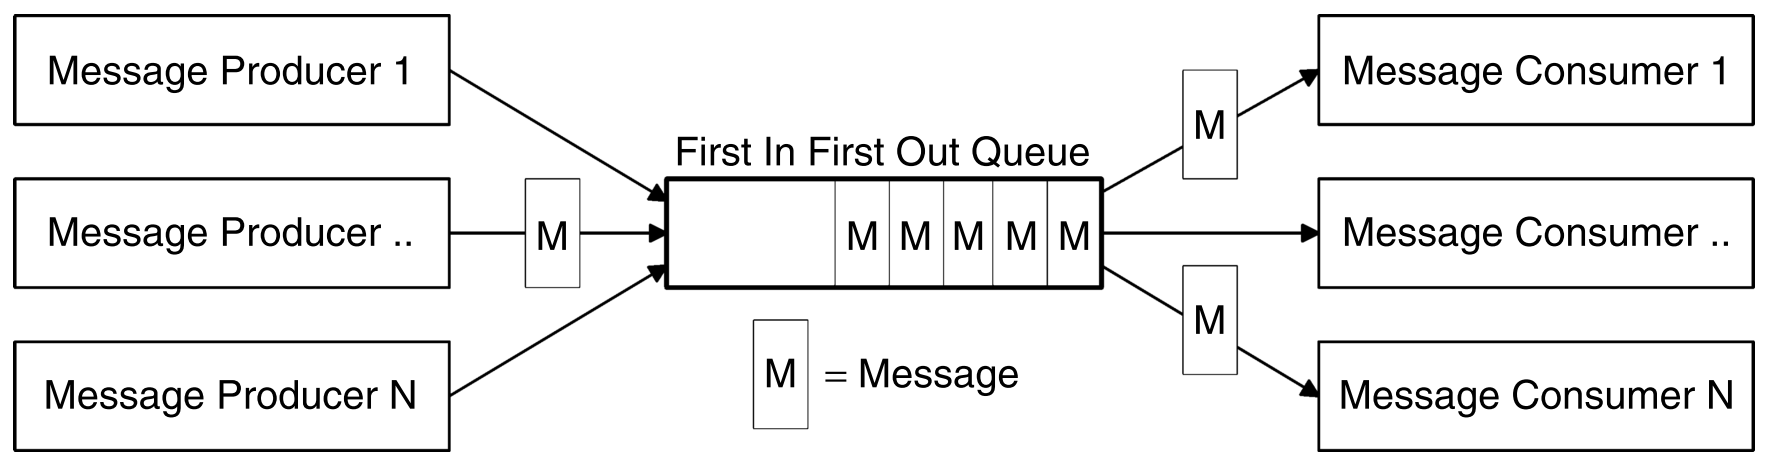
\includegraphics[width=.8\textwidth]{images/middleware_queue.png}
    \caption{A Senerio where Queue is used in Message-Oriented Middleware \cite{CurryMfc2004}}
    \label{fig:diagram}
\end{figure}

The abstract syntax tree of \emph{system}s is shown as follows.
\begin{bnf}
    \ntsym{system} ::= & \tsym{system} \ntsym{template}^?\ntsym{identifier} \tsym{(} \ntsym{port}^* \tsym{)} \tsym{\{}\\
    & (\tsym{internals} \ntsym{identifier}^+)^? \\
    & (\tsym{components} \tsym{\{} \ntsym{componentDecl}^* \tsym{\}})^? \\
    & \tsym{connections} \tsym{\{} \ntsym{connectionDecl}^* \tsym{\}} \tsym{\}}\\
    \ntsym{componentDecl} ::= & \ntsym{identifier}^+ \tsym{:} \ntsym{systemType} \\
    \ntsym{connectionDecl} ::= & \ntsym{systemType} \ntsym{params} \tsym{(} \ntsym{portName}^+ \tsym{)}
\end{bnf}

% The \emph{type} of a system (i.e. its template, name, and ports) shares exactly the same form and meaning with \emph{type} of an automaton. This also suggests that system is NOT a special semantics unit, but simply an compositional approach to pile up automata.
% We declare a system with its template, name and type, then it is implemented by an optional set of \emph{internal node}s, an optional set of \emph{component}s and a set of \emph{connection}s.

\smalltitle{Template} In templates of systems, all parameters types are supported including \emph{a)} parameters of abstract type \texttt{type}, \emph{b)} parameters of primitive types and composite types, and \emph{c)} interfaces and functions.

\smalltitle{Name and Type} Exactly the same with \emph{name} and \emph{type} of an automaton.

\smalltitle{Components} In the \texttt{components} segment, we can declare any entity of an \emph{interface type} as components, e.g. an automaton (see in Example. \ref{exp:middleware_system}), a system, or a parameter of interface type (see in Example. \ref{exp:clustersystem}). 
After being declared, ports of a component can be referenced by \texttt{component.portname}.

\smalltitle{Connections} Connections, e.g. the arrows in Figure. \ref{fig:diagram}, are used to link between \emph{a) the ports of itself, b) the ports of components, and c) the internal nodes}. We declare the connections in the \texttt{connections} segments as shown in Example. \ref{exp:middleware_system}.
Both components and connections are supposed to run parallelly as automata.

\smalltitle{Internals} In certain cases, we need to combine multiple connections to perform more complicated coordination. Internal nodes, as declared in \texttt{internals} segment, are untyped identifiers which are capable to weld two connections.

% Essentially, data flow in an internal node should always follow the same direction, i.e. an internal node doesn't collect or generate any data, it only receives from one end and forward it simultaneously. The direction, together with the type of an internal node, should be determined when being compiled.

\begin{example}[\lang{} Model of the System in Figure. \ref{fig:diagram}] In the previous figure, a simple scenario is presented where a queue is used as a message-oriented middleware. To model this scenario, we need two automata \emph{Producer} and \emph{Consumer} (definitions are omitted due to space limit) that produce or consume message of type \emph{T}.
\begin{lstlisting}
automaton <T:type> Producer (OUT: out T) { ... }
automaton <T:type> Consumer (IN: in T) { ... }

system <T:type> middleware_in_use () {
    components {
        producer_1, producer_2, producer_3 : Producer<T>;
        consumer_1, consumer_2, consumer_3 : Consumer<T>;
    }
    internals  M1, M2 ;
    connections {
        Merger<T>(producer_1.OUT, producer_2.OUT, producer_3.OUT, M1);
        Queue<T>(M1, M2);
        Replicator<T>(M2, consumer_1.IN, consumer_2.IN, consumer_3.IN);
    }
}
\end{lstlisting}
\label{exp:middleware_system}
\end{example}

A system is denoted by a 4-tuple
$S=\langle Ports, Entities, Internals, Links\rangle$ where $Ports$ is a set of ports, $Entities$ is a set of automata or systems (including both components and connections), $Internals$ is a set of internal nodes and $Links$ is a set of pairs, where each element is a port or an internal node. A link $\langle p_1,p_2\rangle$ suggests that $p_1$ and $p_2$ are linked together. A well-defined system satisfies the following assumptions:

% TODO:
\begin{enumerate}
    \item $\forall \langle p_1,p_2\rangle \in Links$, data transfer from $p_1$ to $p_2$. For example, if $p_1\in Ports$ is an input port, $p_2$ could be \emph{a) an output port of the system ($p_2\in Ports$)}, \emph{b) an input port of some automaton $A_i\in Automata$ ($p_2\in A_i.Ports$)} or \emph{c) an internal node ($p_2\in Internals$)}.
    \item $\forall n\in Internals,\exists!p_1,p_2$ i.e. $\langle p_1,n\rangle ,\langle n,p_2\rangle\in Links$ and $p_1,p_2$ have the same data type.
\end{enumerate}

\label{subsec:functions}